\subsubsection{Electrocardiogram (ECG) data}
\label{subsubsec:results_ecg_2}

\paragraph*{Analysis of the heartbeat frequency (BPM)}\mbox{}\\

If the variation between the First and the Return round is positive, it means that the user had an increase on his/her mental workload and vice-versa. Comparing the two groups, the audio method is associated with a slightly lower heart rate for blind people, but the opposite happens for sighted participants. Moreover, data from blind participants have a significant variance. This significant variance can also be observed in the boxplot of Figures \ref{fig:boxplot_ecg_bpm_4_scene} and \ref{fig:boxplot_ecg_bpm_4_rounds}. 

\begin{figure}[!htb]
    \centering
    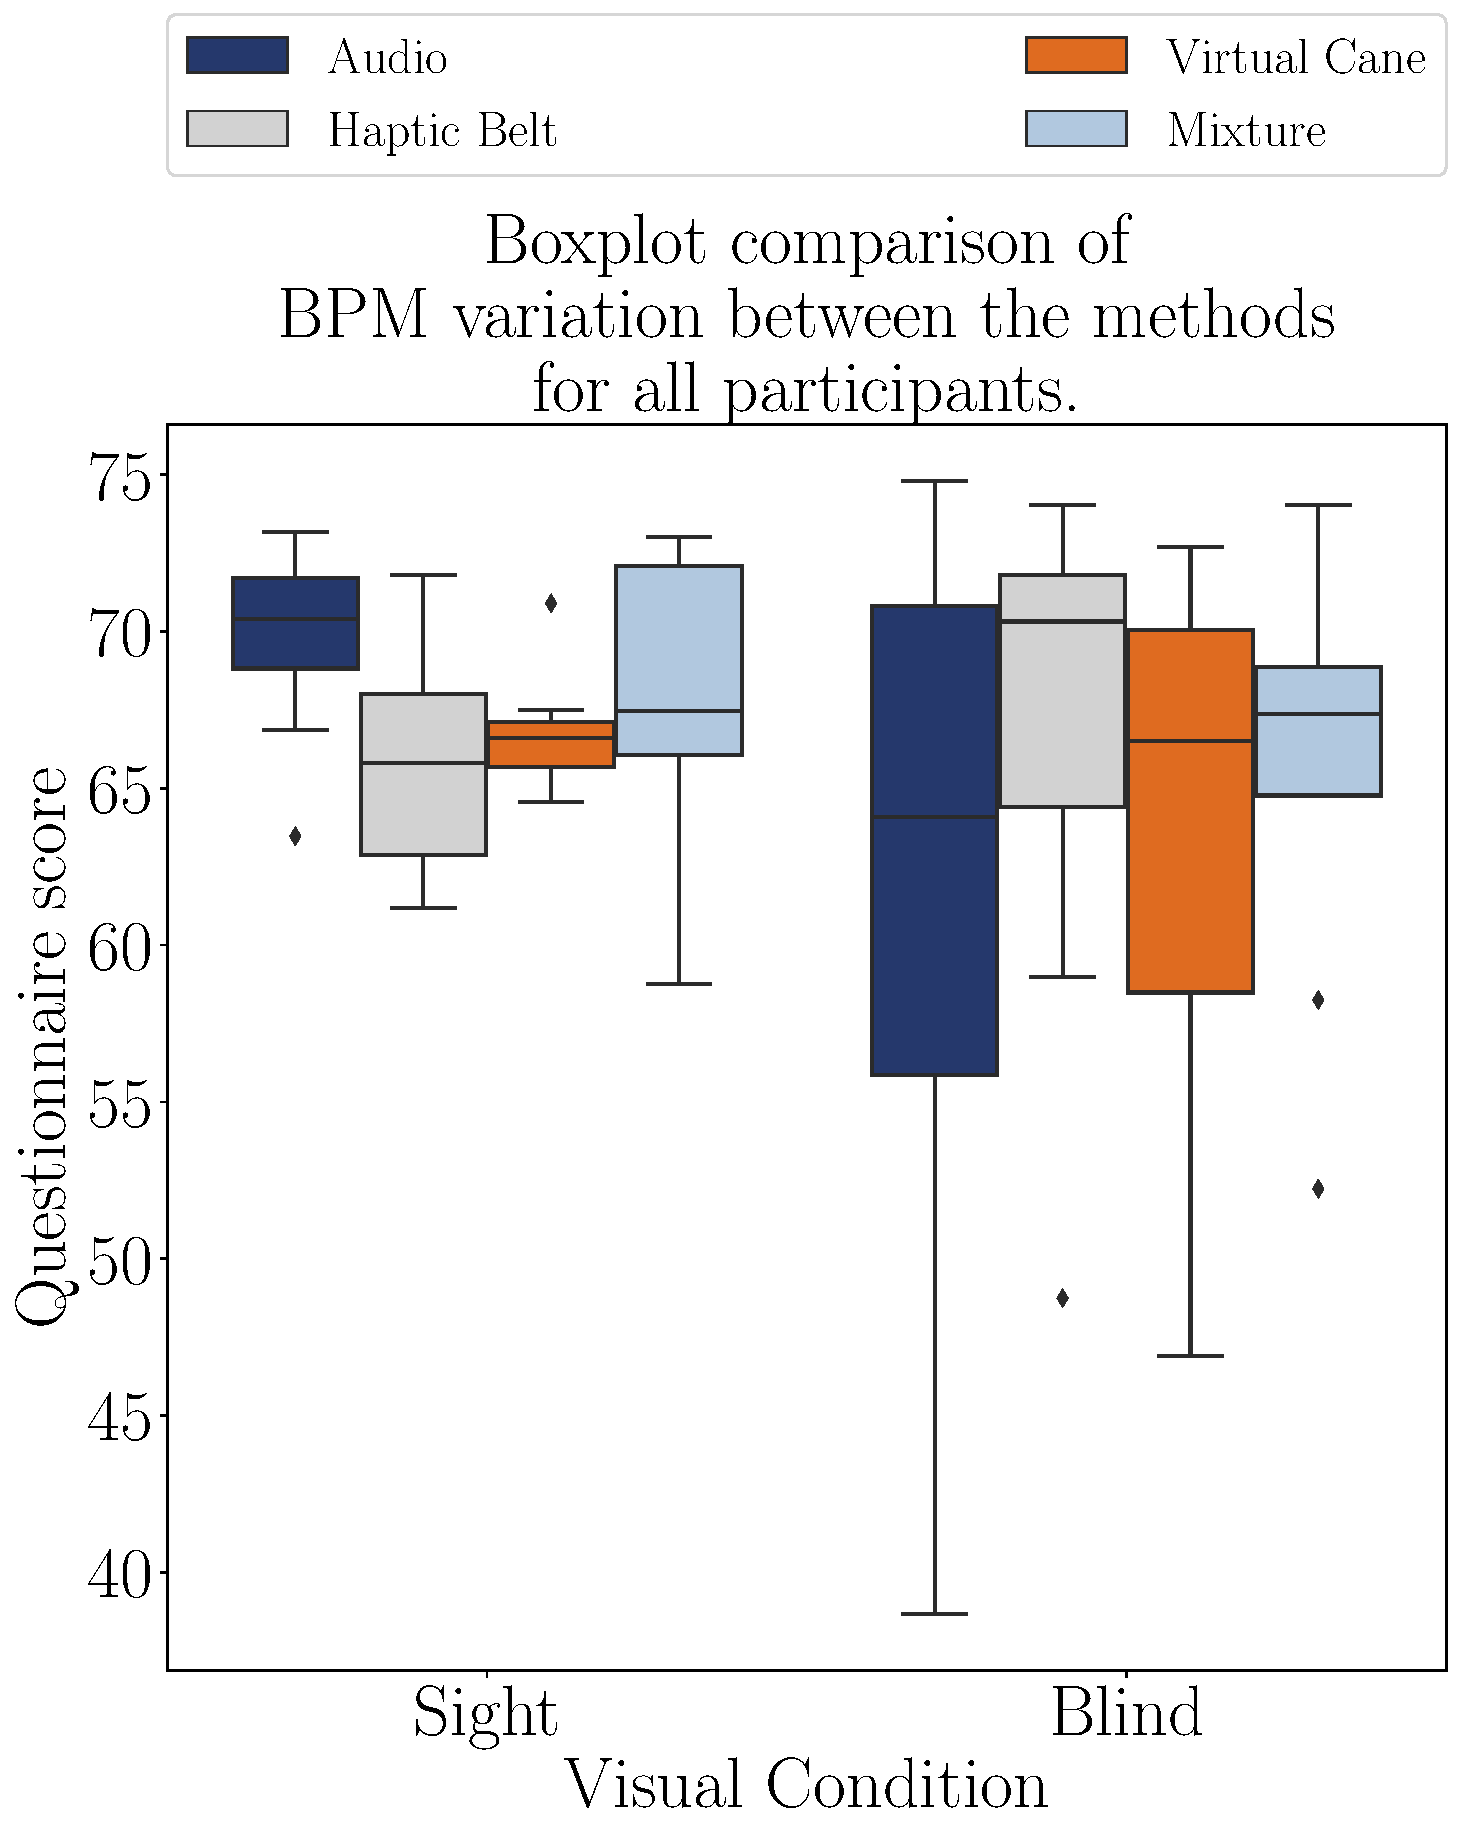
\includegraphics[width = 0.75\linewidth]{3 - Resultados/Figuras/boxplot_ecg_bpm_4_scene.pdf}
    \caption{Boxplot of the average BPM of the participants grouped by the methods.}
    \label{fig:boxplot_ecg_bpm_4_scene}
\end{figure}
\begin{figure}[!htb]
    \centering
    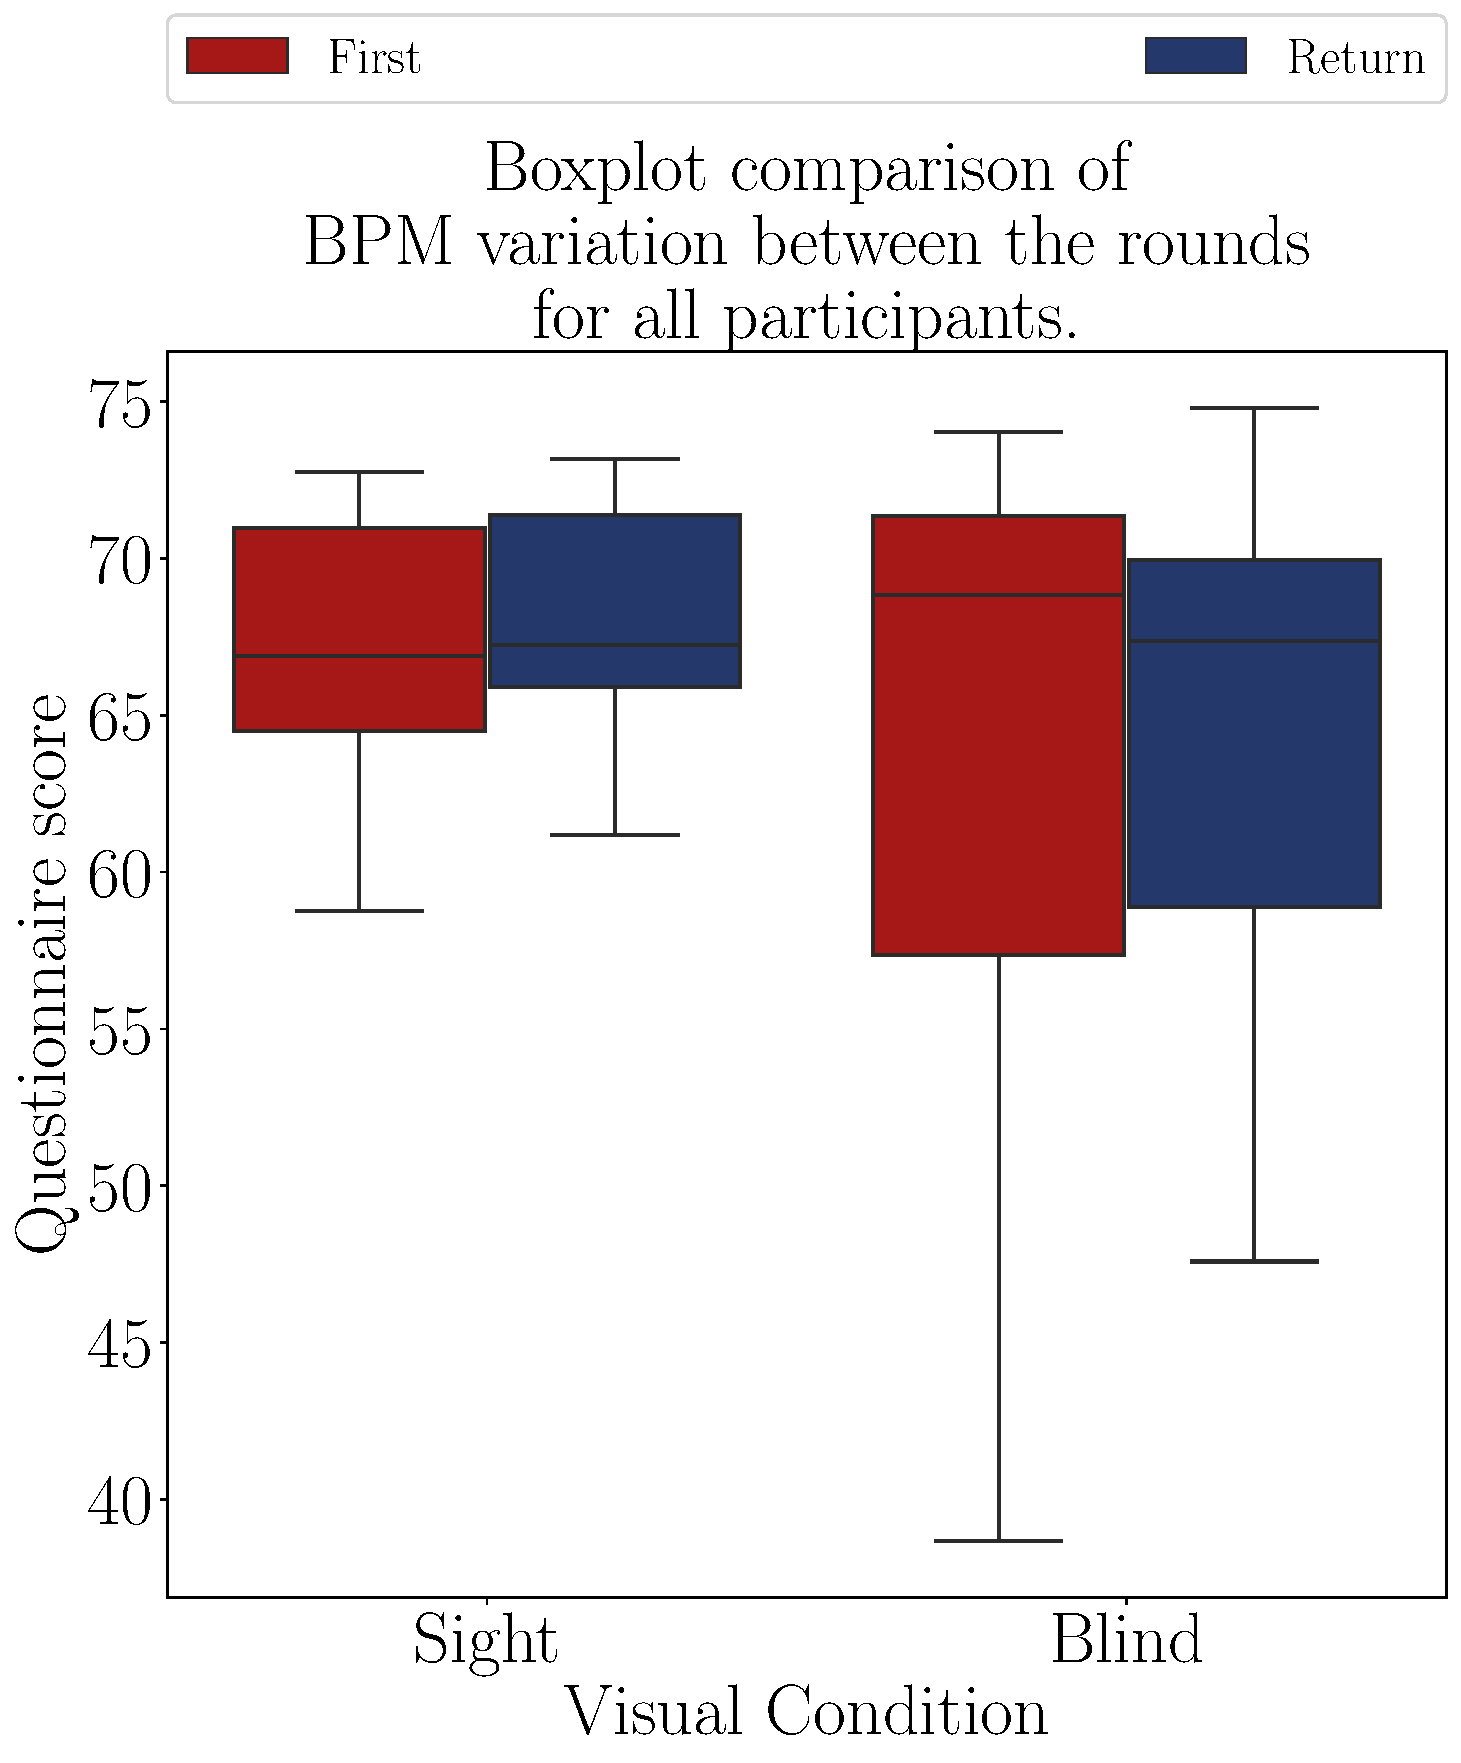
\includegraphics[width = 0.75\linewidth]{3 - Resultados/Figuras/boxplot_ecg_bpm_4_rounds.pdf}
    \caption{Boxplot of the average BPM of the participants grouped by the rounds.}
    \label{fig:boxplot_ecg_bpm_4_rounds}
\end{figure}

Table \ref{tab:blocanova_bpm_two_way_blind_sight} brings the results from ANOVA, which are similar for both sighted and blind participants.

\begin{table}[!htb]
    \caption{Anova p-value for the BPM on each method.}
    \label{tab:blocanova_bpm_two_way_blind_sight}
\begin{minipage}{0.45\linewidth}
    \subcaption{Blind participants}
    \input{3 - Resultados/Tabelas/blocanova_bpm_two_way_blindsemBegin.tex}
\end{minipage}%
\begin{minipage}{0.05\linewidth}
    \hfill
\end{minipage}%
\begin{minipage}{0.45\linewidth}
    \subcaption{Sight participants}
    \input{3 - Resultados/Tabelas/blocanova_bpm_two_way_sightsemBegin.tex}
\end{minipage}
\end{table}


%%%%%%%%%%%%%%%%%%%%%%%%%%%%%%%%%%%%%%%%%%%%%%%%%%%%%%%%%%%%%%%%%%%%%%%%%%%%
%%%%%%%%%%%%%%%%%%%%%%%%%%%%%%%%%%%%%%%%%%%%%%%%%%%%%%%%%%%%%%%%%%%%%%%%%%%%
%%%%%%%%%%%%%%%%%%%%%%%%%%%%%%%%%%%%%%%%%%%%%%%%%%%%%%%%%%%%%%%%%%%%%%%%%%%%
%%%%%%%%%%%%%%%%%%%%%%%%%%%%%%%%%%%%%%%%%%%%%%%%%%%%%%%%%%%%%%%%%%%%%%%%%%%%

\paragraph*{Analysis of the heartbeat variance (SDNN)}\mbox{}\\

Figures \ref{fig:boxplot_ecg_sdnn_4_scene} and \ref{fig:boxplot_ecg_sdnn_4_rounds} shows the boxplots for both groups. Both pictures show that the SDNN of the sighted users was higher than that of the blind users, indicating that sighted users had a lower mental workload than the blind users.

\begin{figure}[!htb]
    \centering
    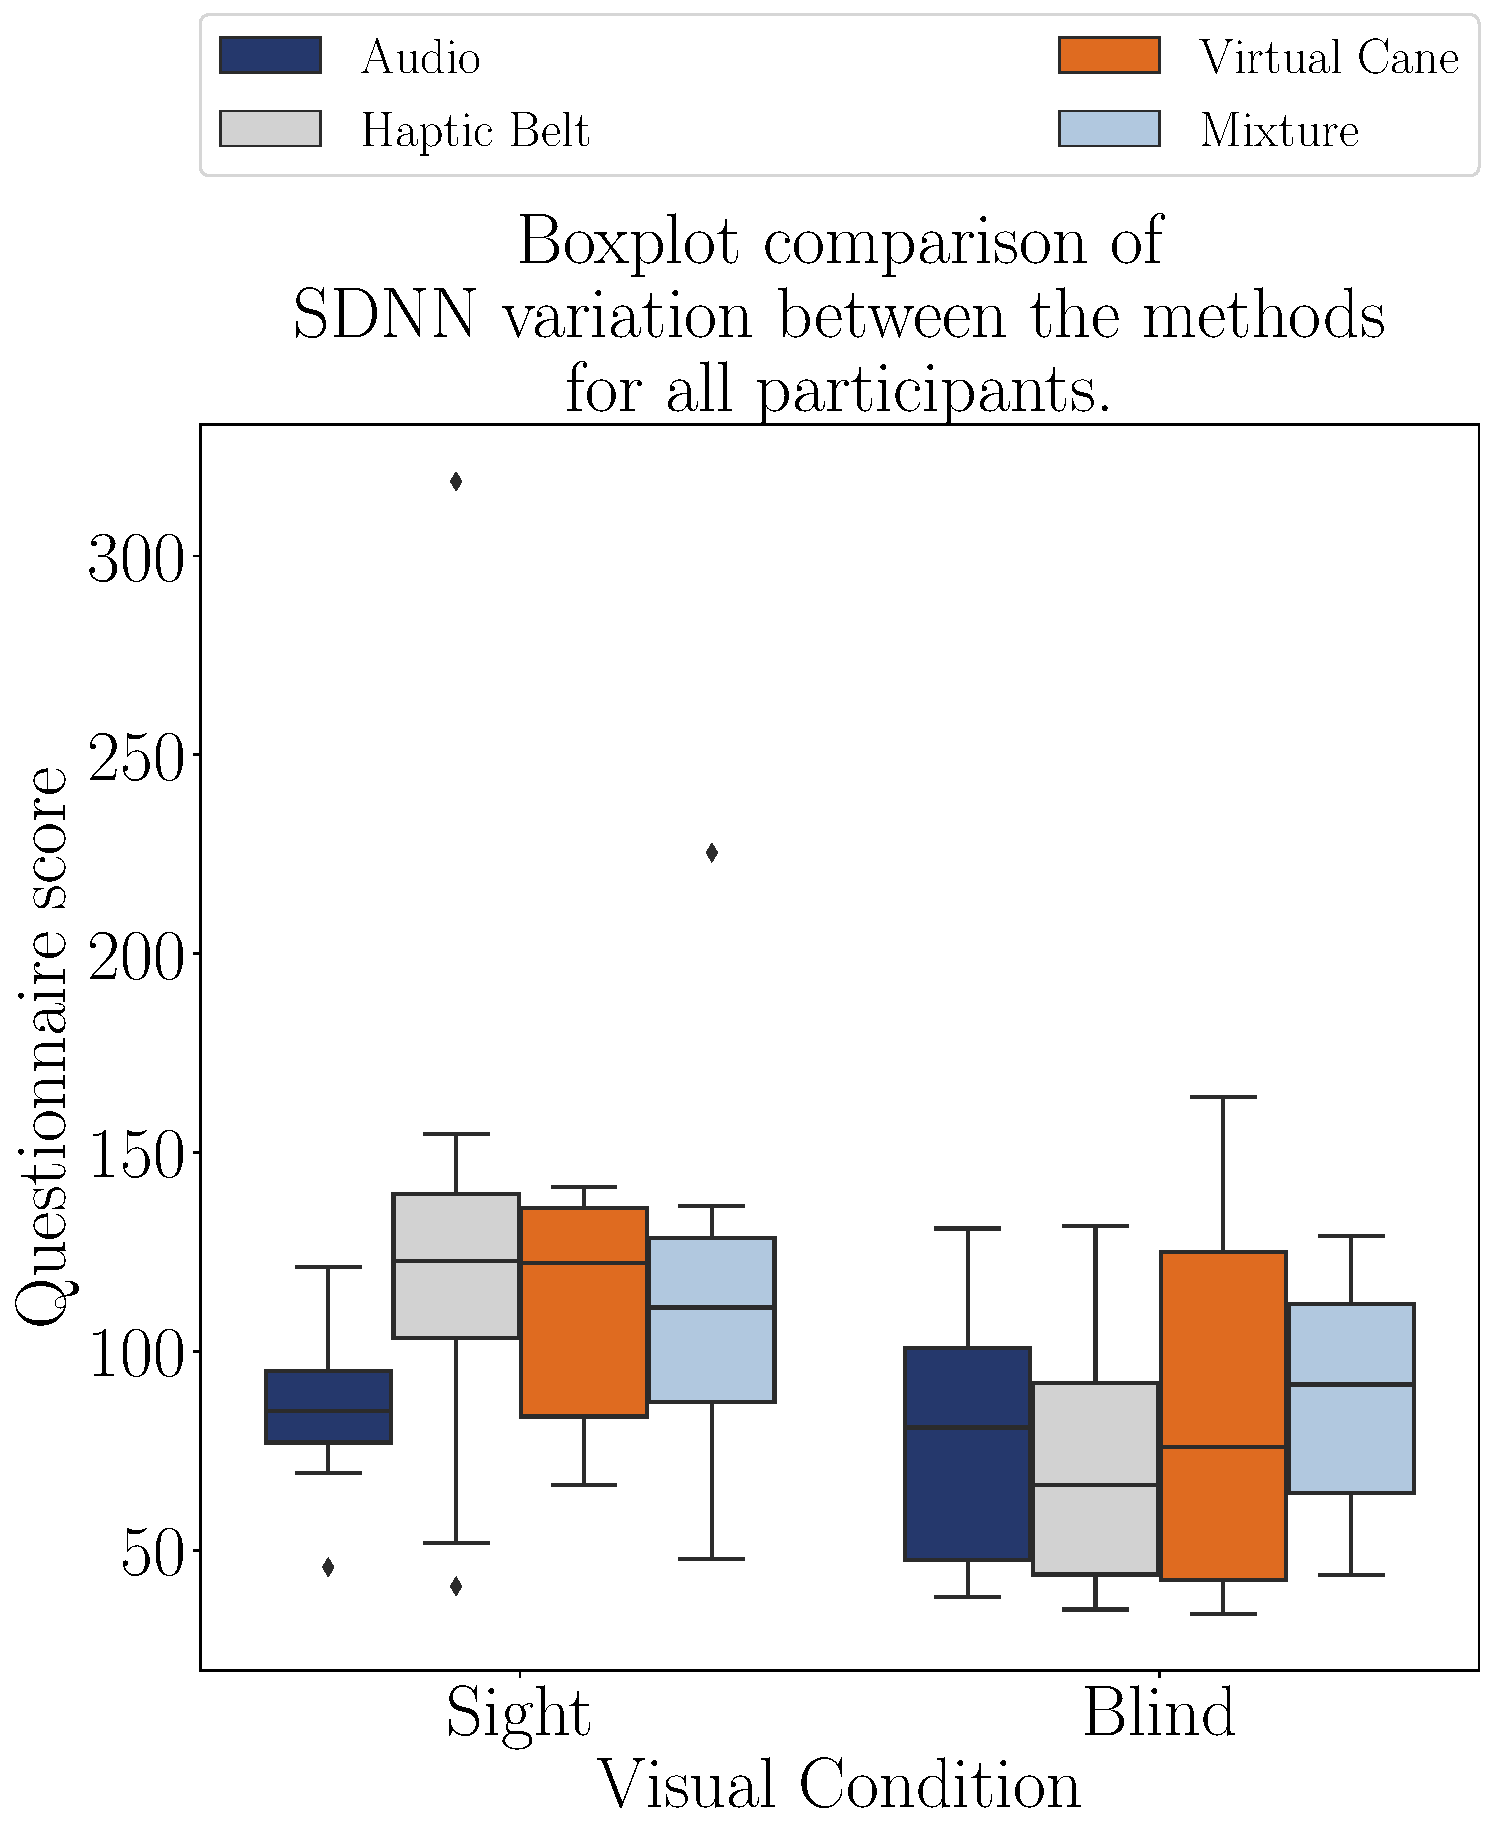
\includegraphics[width = 0.75\linewidth]{3 - Resultados/Figuras/boxplot_ecg_sdnn_4_scene.pdf}
    \caption{Boxplot of the average SDNN of the participants grouped by the methods.}
    \label{fig:boxplot_ecg_sdnn_4_scene}
\end{figure}
\begin{figure}[!htb]
    \centering
    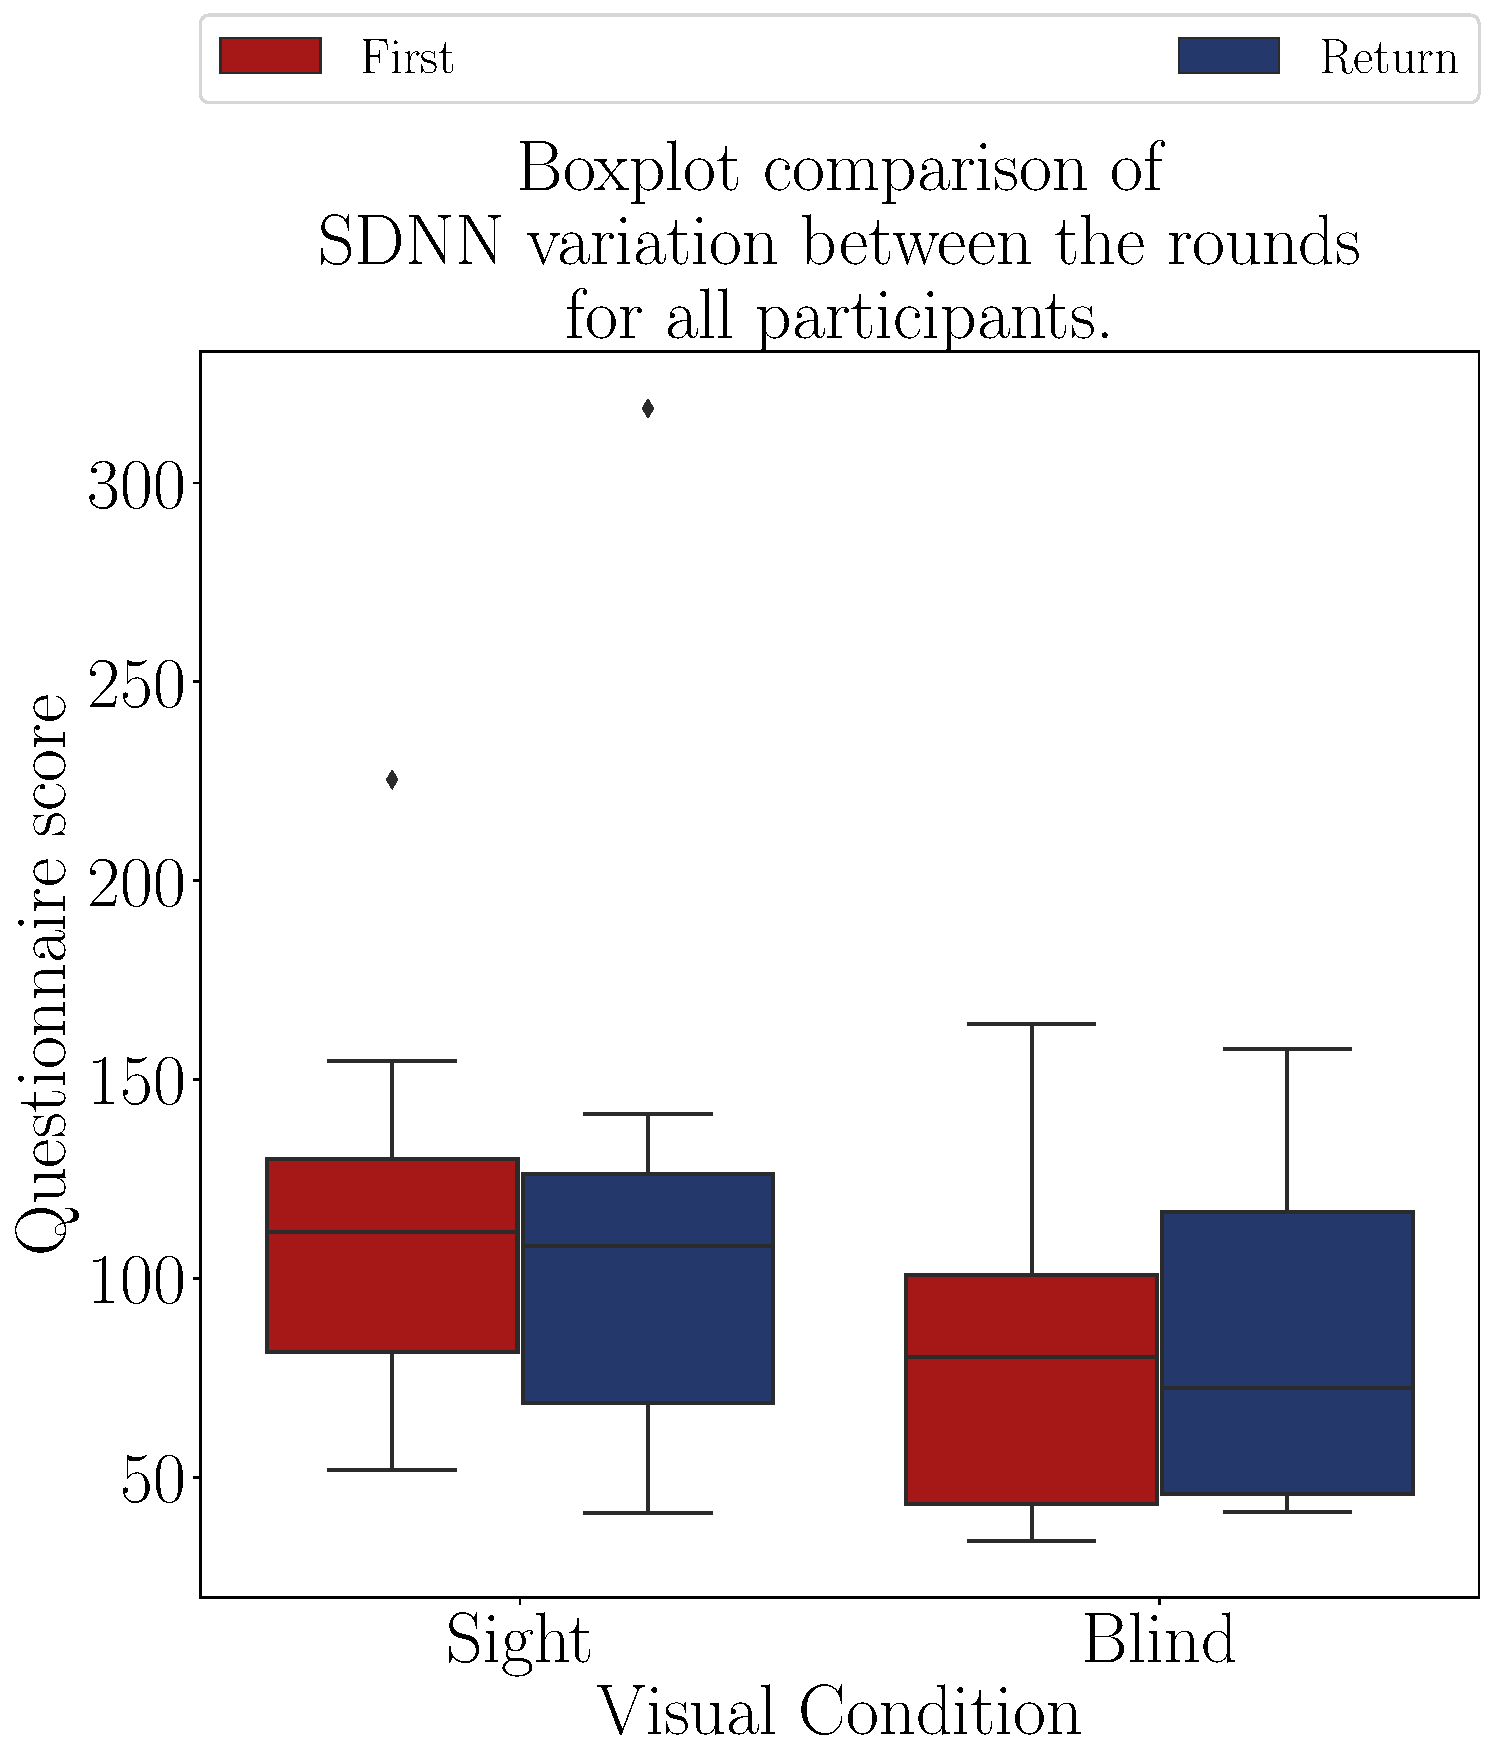
\includegraphics[width = 0.75\linewidth]{3 - Resultados/Figuras/boxplot_ecg_sdnn_4_rounds.pdf}
    \caption{Boxplot of the average SDNN of the participants grouped by the rounds.}
    \label{fig:boxplot_ecg_sdnn_4_rounds}
\end{figure}
 
Table \ref{tab:blocanova_sdnn_two_way_blind_sight} shows the ANOVA test p-values. For both groups, none of the factors have a significant influence on the SDNN value.

\begin{table}[!htb]
    \caption{Anova p-value for the average SDNN on each method.'}
    \label{tab:blocanova_sdnn_two_way_blind_sight}
\begin{minipage}{0.45\linewidth}
    \subcaption{Blind participants}
    \input{3 - Resultados/Tabelas/blocanova_sdnn_two_way_blindsemBegin.tex}
\end{minipage}%
\begin{minipage}{0.05\linewidth}
    \hfill
\end{minipage}%
\begin{minipage}{0.45\linewidth}
    \subcaption{Sight participants}
    \input{3 - Resultados/Tabelas/blocanova_sdnn_two_way_sightsemBegin.tex}
\end{minipage}
\end{table}